\section{Problema 1: validación del servidor CI/CD M/M/1}

\subsection{Parámetros y justificación del modelo}

Los registros indican un trabajo cada 4 minutos en promedio, es decir,
$\lambda=0{,}25$ trabajos/min, y una duración media de servicio de 3 minutos,
$\mu=1/3$ trabajos/min. Los tiempos entre llegadas son exponenciales
(proceso Poisson), los servicios son exponenciales, hay un único servidor, la
disciplina es FIFO y la cola es prácticamente ilimitada. Esas cuatro
propiedades definen un M/M/1. La Tabla~\ref{tab:mm1-parametros} resume los
parámetros y las cantidades analíticas.

\begin{table}[H]
\centering
\small
% Tabla generada automáticamente por simulacion_colas.report.
% No editar a mano: regenerar con `python -m simulacion_colas report`.
\begin{tabular}{lrl}
\toprule
Parámetro & Valor & Unidad \\
\midrule
Tasa de llegadas $\lambda$ & 0,2500 & trabajos/min \\
Tasa de servicio $\mu$ & 0,3333 & trabajos/min \\
Utilización $\rho=\lambda/\mu$ & 0,7500 & -- \\
Número medio en el sistema $L$ & 3,0000 & trabajos \\
Número medio en cola $L_q$ & 2,2500 & trabajos \\
Tiempo medio en el sistema $W$ & 12,0000 & min \\
Tiempo medio en cola $W_q$ & 9,0000 & min \\
\bottomrule
\end{tabular}

\caption{Parámetros y valores analíticos del servidor CI/CD M/M/1.}
\label{tab:mm1-parametros}
\end{table}

\subsection{Warm-up}

La Tabla~\ref{tab:warmup} muestra el piloto de período transitorio. Las
diferencias de $L$ y $W$ respecto de la corrida de 5\,000 minutos ya son
inferiores al $0{,}5$\,\% desde 1\,000 minutos; por eso se adopta ese warm-up.
El valor de 1\,000 minutos se resalta en negrita.

\begin{table}[H]
\centering
\small
% Tabla generada automáticamente por simulacion_colas.report.
% No editar a mano: regenerar con `python -m simulacion_colas report`.
\begin{tabular}{rrrrr}
\toprule
Warm-up (min) & $L$ & $W$ (min) & $\Delta L$ (\%) & $\Delta W$ (\%) \\
\midrule
0 & 3,0226 & 12,0920 & -1,246 & -1,194 \\
500 & 3,0287 & 12,1231 & -1,046 & -0,940 \\
\textbf{1.000} & 3,0454 & 12,1883 & -0,499 & -0,407 \\
2.000 & 3,0503 & 12,2065 & -0,339 & -0,258 \\
5.000 & 3,0607 & 12,2381 & 0,000 & 0,000 \\
\bottomrule
\end{tabular}

\caption{Piloto de warm-up del M/M/1 con 10 réplicas por candidato.}
\label{tab:warmup}
\end{table}

\subsection{Resultados y validación}

La Tabla~\ref{tab:mm1-validacion} compara las estimaciones con las fórmulas
analíticas. Los cinco intervalos de confianza del 95\,\% contienen su valor
teórico. Los errores relativos van de $0{,}5$\,\% a $3{,}2$\,\%, valores
razonables para un horizonte de 30\,000 minutos. La Figura~\ref{fig:mm1}
presenta la comparación gráfica y el piloto de warm-up.

\begin{table}[H]
\centering
\small
% Tabla generada automáticamente por simulacion_colas.report.
% No editar a mano: regenerar con `python -m simulacion_colas report`.
\begin{tabular}{llrrrl}
\toprule
Métrica & Unidad & Media & IC95\,\% & Analítico & ¿Contiene? \\
\midrule
$L$ & trabajos & 3,0466 & [2,9712; 3,1220] & 3,0000 & Sí \\
$L_q$ & trabajos & 2,2961 & [2,2234; 2,3689] & 2,2500 & Sí \\
$W$ & min & 12,2045 & [11,9197; 12,4892] & 12,0000 & Sí \\
$W_q$ & min & 9,1973 & [8,9186; 9,4760] & 9,0000 & Sí \\
$\rho$ & -- & 0,7505 & [0,7470; 0,7540] & 0,7500 & Sí \\
\bottomrule
\end{tabular}

\caption{Validación del M/M/1 con 50 réplicas, warm-up de 1\,000 min y horizonte de 30\,000 min.}
\label{tab:mm1-validacion}
\end{table}

\begin{figure}[H]
\centering
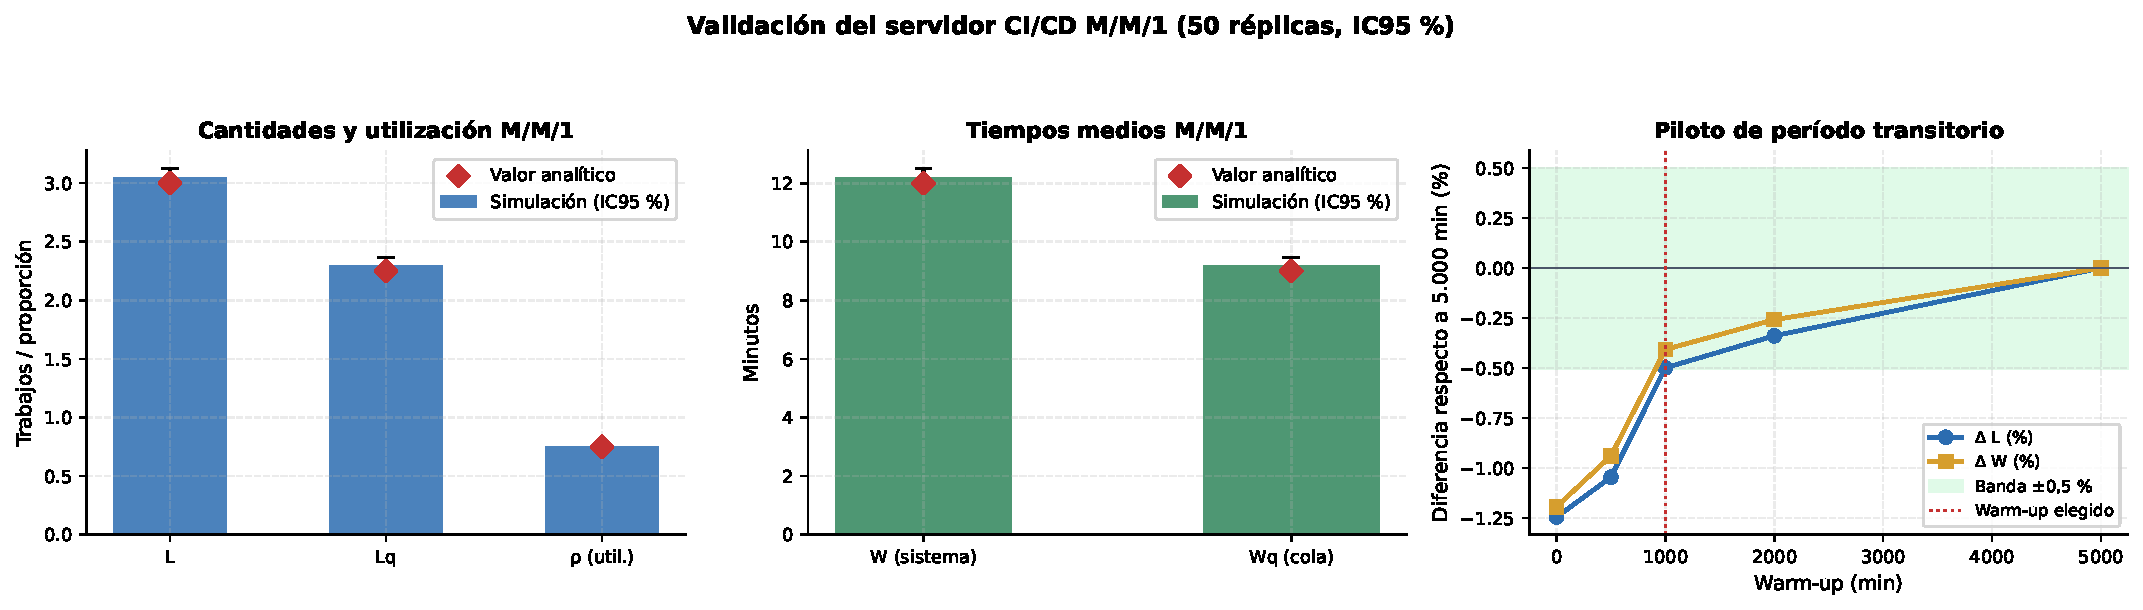
\includegraphics[width=\linewidth]{mm1_validation.pdf}
\caption{Validación del M/M/1: cantidades medias, tiempos medios y piloto de warm-up.}
\label{fig:mm1}
\end{figure}

La Ley de Little se cumple numéricamente: los cocientes
$L/(\lambda W)$ y $L_q/(\lambda W_q)$ son $0{,}999997$ y $0{,}999978$,
respectivamente, es decir, difieren de la unidad en menos de $0{,}003$\,\%.
Esto confirma la consistencia interna del simulador y la correcta
implementación de los acumuladores.
